{\begin{center}
  \resizebox{0.8\columnwidth}{!}{%
    \begin{tikzpicture}
    %\draw (0,0) --(1,2);
    \draw (-1.8, -9.8) node[inner sep=0] {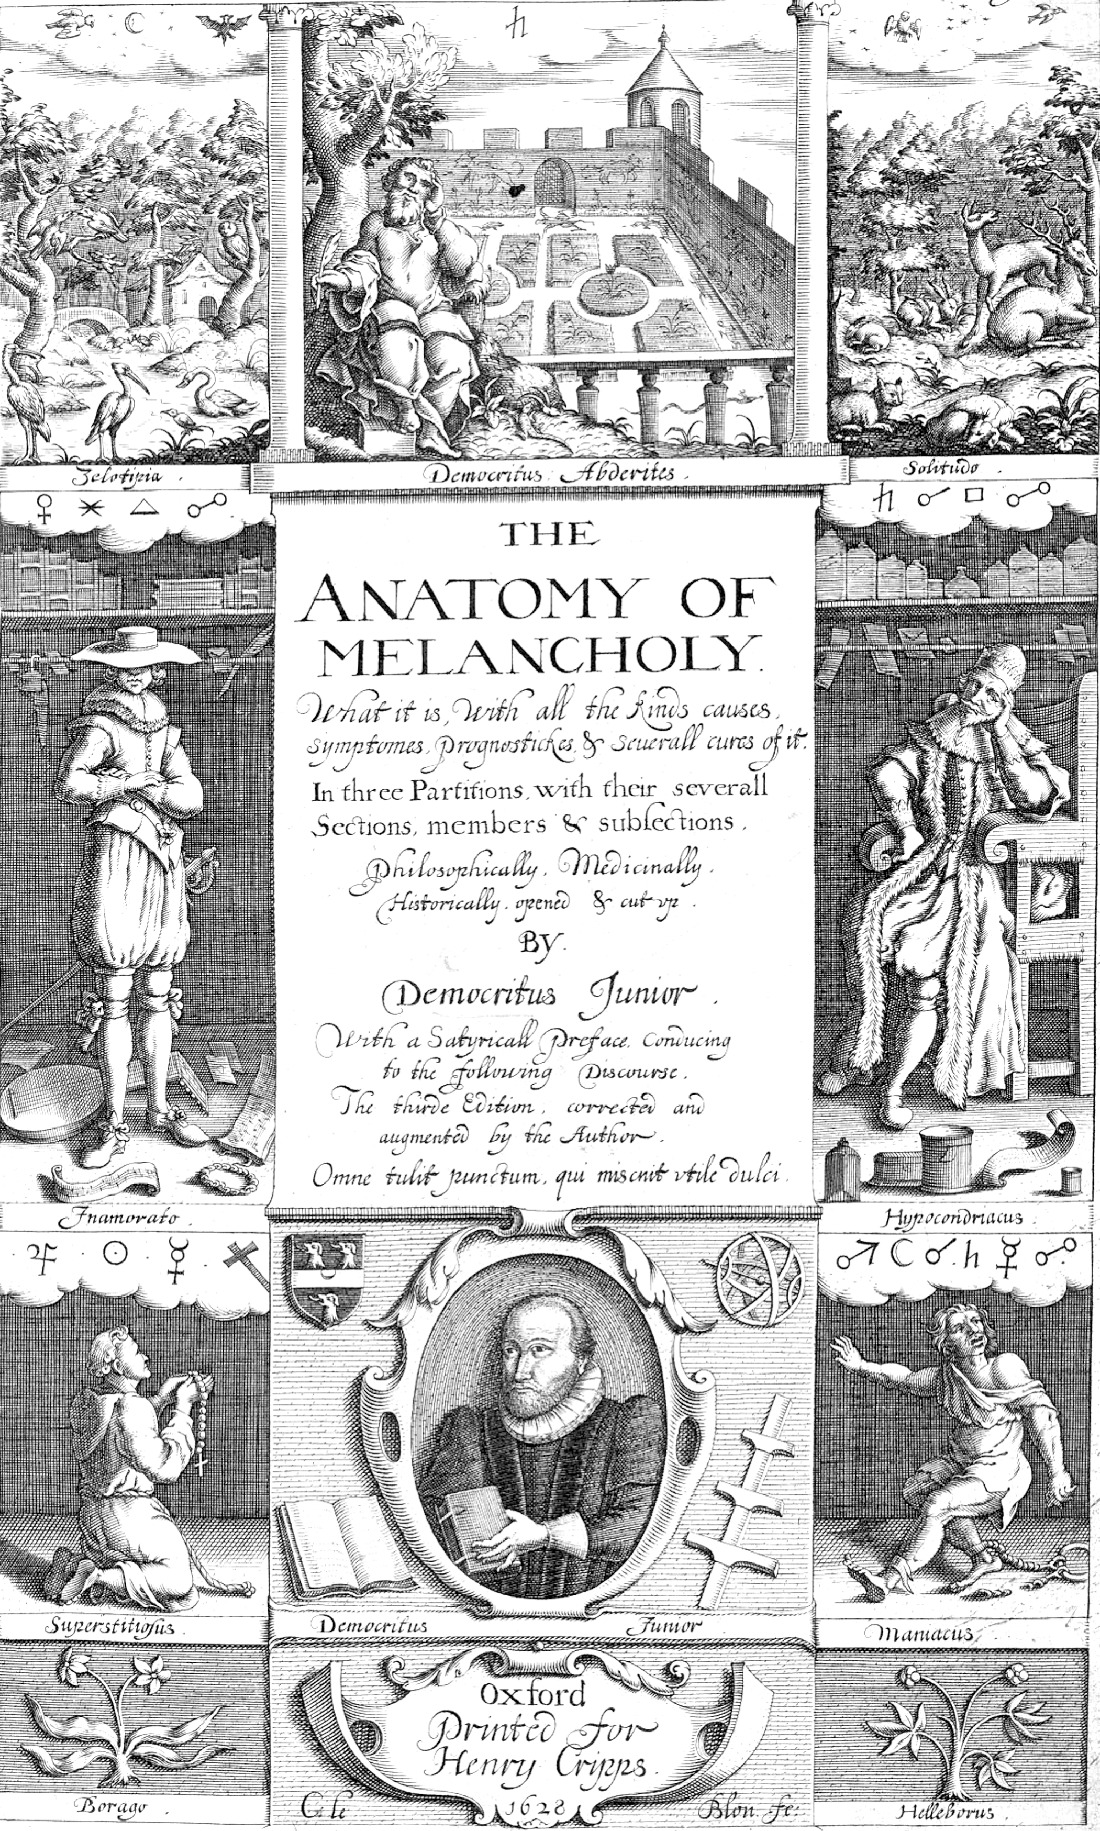
\includegraphics[height=0.6\paperheight]{frontispiece.jpg}};
    %\node [fill=white, red] at (1,-12.5) {8helle}; % helleborus
      %\node [fill=white, red] at (1.6,-11) {7maniac}; % maniacus
      %\node [fill=white, red] at (1.6,-7) {5hypoc}; % Hypocondriacus
      %\node [fill=white, red] at (1.6,-4.3) {3solitudo}; % Solitudo
      %\node [fill=white, red] at (-3.2,-11) {6supersti}; % Superstitiosus
      %\node [fill=white, red] at (-3.2,-7.5) {4inamor}; % Inamorato
      %\node [fill=white, red] at (-2.8,-4) {2jealous}; % Jealous
      %\node [fill=white, red] at (-1,-3.5) {1democr}; % Democritus
      \node[align=left] at (-1.0,0.0) {Old \textsc{Democritus} under a tree,\\Sits on a stone with book on knee;\\About him hang there many features,\\Of Cats, Dogs and such like creatures,\\Of which he makes anatomy,\\The seat of black choler to see.\\Over his head appears the sky,\\And Saturn Lord of melancholy.};
    \node[align=left] at (5.9,0.0) {To the left a landscape of \textsc{Jealousy},\\Presents itself unto thine eye.\\A Kingfisher, a Swan, an Hern,\\Two fighting-cocks you may discern,\\Two roaring Bulls each other hie,\\To assault concerning venery.\\Symbols are these; I say no more,\\Conceive the rest by that’s afore.};
    \node[align=left] at (6,-4.2) {The next of \textsc{solitariness},\\A portraiture doth well express,\\By sleeping dog, cat: Buck and Doe,\\Hares, Conies in the desert go:\\Bats, Owls the shady bowers over,\\In melancholy darkness hover.\\Mark well: If’t be not as’t should be,\\Blame the bad Cutter, and not me.};
    \node[align=left] at (6,-8.5) {I’th’ under column there doth stand\\\textsc{Inamorato} with folded hand;\\Down hangs his head, terse and polite,\\Some ditty sure he doth indite.\\His lute and books about him lie,\\As symptoms of his vanity.\\If this do not enough disclose,\\To paint him, take thyself by th’ nose.};

    \node[align=left] at (6,-12.7) {\textsc{Hypocondriacus} leans on his arm,\\Wind in his side doth him much harm,\\And troubles him full sore, God knows,\\Much pain he hath and many woes.\\About him pots and glasses lie,\\Newly brought from’s Apothecary.\\This Saturn’s aspects signify,\\You see them portray’d in the sky.};

    \node[align=left] at (5.9,-17) {Beneath them kneeling on his knee,\\A \textsc{superstitious} man you see:\\He fasts, prays, on his Idol fixt,\\Tormented hope and fear betwixt:\\For Hell perhaps he takes more pain,\\Than thou dost Heaven itself to gain.\\Alas poor soul, I pity thee,\\What stars incline thee so to be?};

    \node[align=left] at (6,-21.5) {But see the \textsc{madman} rage downright\\With furious looks, a ghastly sight.\\Naked in chains bound doth he lie,\\And roars amain he knows not why!\\Observe him; for as in a glass,\\Thine angry portraiture it was.\\His picture keeps still in thy presence;\\’Twixt him and thee, there’s no difference.};

    \node[align=left] at (-1.8,-20.0) {\textsc{Borage} and \textsc{Hellebor} fill two scenes,\\Sovereign plants to purge the veins\\Of melancholy, and cheer the heart,\\Of those black fumes which make it smart;\\To clear the brain of misty fogs,\\Which dull our senses, and Soul clogs.\\The best medicine that e’er God made\\For this malady, if well assay’d.};

    % 1 - Democritus arrows
      \draw [ultra thick, black] (-4.3, 2.1) rectangle (2.2,-2.1); % text box
      \draw [ultra thick, black] (-1.8, -2.1) -- (-1.8,-4.1); %arrow
      \draw [ultra thick, black] (-3.3, -7.1) rectangle (-0.2,-4.1); % map box
      \fill [nearly transparent, black] (-3.3, -7.1) rectangle (-0.2,-4.1); % map box

      % 2 - Jealousy arrows
      \draw [ultra thick, dashed, red] (2.7, -2) -- (2.7,-3); %
      \draw [ultra thick, dashed, red] (-4.5, -3) -- (2.7,-3); %
      \draw [ultra thick, dashed, red] (-4.5, -3) -- (-4.5,-4); %
      % 2 - Jealousy box
      \fill[nearly transparent, red] (-5.3,-4)rectangle(-3.5,-7);
      \draw [ultra thick, dashed, red](2.7,-2)rectangle(9,2.2);
      \draw [ultra thick, dashed, red](-5.3,-4)rectangle(-3.5,-7);


      % 3 - Solitudo arrows
      \draw [ultra thick, black] (2.9, -6.3) rectangle (9.2,-2.2); % text box
      \draw [ultra thick, black] (1.6, -5.5) -- (2.9,-5.5); %
      \draw [ultra thick, black](1.6,-4.1)rectangle(-0.1,-7.1); % map box
      \fill [nearly transparent, black](1.6,-4.1)rectangle(-0.1,-7.1); % map box

      % 4 - Inamorato arrows
      \draw [ultra thick, dashed, red] (-3.5, -8.2) -- (2.8,-8.2); % arrow
      % 4 - Inamorato box
      \fill[nearly transparent, red] (-5.3,-7.2)rectangle(-3.5,-11.5);
      \draw [ultra thick, dashed, red](2.7,-10.5)rectangle(9.3,-6.4);
      \draw [ultra thick, dashed, red](-5.3,-7.2)rectangle(-3.5,-11.5);


      % 5 - Hypocondriacus arrows
      \draw [ultra thick, black] (1.6, -9.3) -- (2.5,-9.3); %
      \draw [ultra thick, black] (2.5, -9.3) -- (2.5,-12.8); %
      \draw [ultra thick, black] (2.5, -12.8) -- (2.7,-12.8); %
      \draw [ultra thick, black](1.6,-7.2)rectangle(-0.1,-11.7); % map box
      \fill [nearly transparent, black](1.6,-7.2)rectangle(-0.1,-11.7); % map box
      \draw [ultra thick, black](2.7,-14.8)rectangle(9.3,-10.7); % text box

      % 6 - Superstitiosus arrows
      \draw [ultra thick, dashed, red] (-5.5, -16.5) -- (2.7,-16.5); %
      \draw [ultra thick, dashed, red] (-5.5, -16.5) -- (-5.5,-13); %
      \draw [ultra thick, dashed, red] (-5.5, -13) -- (-5.3,-13); %
      % 6 - Superstitiosus box
      \fill[nearly transparent, red](-5.3,-11.8)rectangle(-3.5,-14.4);
      \draw [ultra thick, dashed, red](-5.3,-11.8)rectangle(-3.5,-14.4);
      \draw [ultra thick, dashed, red](2.7,-19.1)rectangle(9.1,-14.9); % text box


      % 7 - Maniac arrows
      \draw [ultra thick, black] (2.2, -23.5) -- (2.4,-23.5); %base
      \draw [ultra thick, black] (2.2, -12.8) -- (2.2,-23.5); %
      \draw [ultra thick, black] (1.6, -12.8) -- (2.2,-12.8); %
      \draw [ultra thick, black](2.4,-23.8)rectangle(9.6,-19.3); % text box
      \draw [ultra thick, black](1.6,-14.4)rectangle(-0.1,-11.8); % map box
      \fill [nearly transparent, black](1.6,-14.4)rectangle(-0.1,-11.8); % map box

      % 8 - Hellebor arrows
      \draw [ultra thick, black] (-2, -15.8) -- (-2,-17.6); %
      \draw [ultra thick, black] (-4.2, -15.8) -- (1,-15.8); %base
      \draw [ultra thick, black] (-4.2, -15.8) -- (-4.2,-15.6); %l
      \draw [ultra thick, black] (1, -15.8) -- (1,-15.6); %base
      % 8 - Hellebore box
      \draw [ultra thick, black](-5.6,-17.6)rectangle(1.9,-22.3);
      \draw [ultra thick, black](-5.2,-14.4)rectangle(-3.5,-15.5); % left map box
      \fill [nearly transparent, black](-5.2,-14.4)rectangle(-3.5,-15.5); % left map box
      \draw [ultra thick, black](-0.1,-14.4)rectangle(1.6,-15.5); % right map box
      \fill [nearly transparent, black](-0.1,-14.4)rectangle(1.6,-15.5); % right map box

    \end{tikzpicture}
  }
  \end{center}
}
